\documentclass[conference]{IEEEtran}
\IEEEoverridecommandlockouts
% The preceding line is only needed to identify funding in the first footnote. If that is unneeded, please comment it out.
\usepackage{cite}
\usepackage{amsmath,amssymb,amsfonts}
\usepackage{algorithmic}
\usepackage{graphicx}
\usepackage{textcomp}
\usepackage{xcolor}
\def\BibTeX{{\rm B\kern-.05em{\sc i\kern-.025em b}\kern-.08em
    T\kern-.1667em\lower.7ex\hbox{E}\kern-.125emX}}
\begin{document}

\title{Automated 4-Way-Road Cross Section}


\author{\IEEEauthorblockN{1\textsuperscript{st} Vytaras Juraska}
\IEEEauthorblockA{\textit{Electronic Engineering} \\
\textit{Hochschule Hamm-Lippstadt}\\
Lippstadt, Germany \\
vytaras.juraska@stud.hshl.de}
\and
\IEEEauthorblockN{2\textsuperscript{nd} Gordan Konevski}
\IEEEauthorblockA{\textit{Electronic Engineering} \\
\textit{Hochschule Hamm-Lippstadt}\\
Lippstadt, Germany \\
gordan.konevski@stud.hshl.de}
\and
\IEEEauthorblockN{3\textsuperscript{rd} Giuseppe Scalora}
\IEEEauthorblockA{\textit{Electronic Engineering} \\
\textit{Hochschule Hamm-Lippstadt}\\
Lippstadt, Germany \\
giuseppe.scalora@stud.hshl.de}
\and
\IEEEauthorblockN{4\textsuperscript{th} Adam Sulak}
\IEEEauthorblockA{\textit{Electronic Engineering} \\
\textit{Hochschule Hamm-Lippstadt}\\
Lippstadt, Germany \\
adam.sulak@stud.hshl.de}

}

\maketitle

\begin{abstract}

\end{abstract}

\section{Introduction}
Road transport automation has the sole purpose of contributing to the key objectives of the EU transport policies, mostly to increase safety, efficiency of traffic, avoidance of traffic congestion on intersections and improve the time frames necessary to do all of this. Beside these formal aspects, some social aspects are covered, for example the improvements in comfort from the users end including elderly people and impaired people.
The automation discussed in this context encapsulates the applications of autonomous driving and interactions/interfacing with an intelligent environment. This last concept must take care of vehicle to vehicle communication and vehicle to infrastructure communication. Many factors can also be taken into consideration when working within the infrastructure context, such as like traffic controllers, traffic lights, pedestrian crossing sections, which all together make for a perfect real environment. Many applications of autonomous driving are already on the road but when it comes to connect this to infrastructure interactions, the technological advancement has still a lot of work to do, despite that, it is commonly accepted that automation in this field will become a reality sooner or later and that it will play a key role in future transport systems. 

\section{Motivation}
The purpose defined for this scope deals with the search and development of a solution to manage the traffic of autonomous cars inside a crossroad-section. It is important to consider the behaviour of these autonomous vehicles in any considered scenario and model the reactions and most efficient ways to deal with the queuing and scheduling of each vehicle in order to accept them by the environment and fluently guide them out of the cross-section in complete safety. This project study will assume that the cross-section handled starts from a well defined distance and that individual sensors, for the autonomous driving of each car, are already handled by the manufacturers. 

\section{Analysis of the problem}
In the problem analysis it is important to define what exactly is there to solve and develop. In order to understand this, it is helpful to take a look at how a real life cross-section behaves and looks like. The main concern is how to accept and register cars that wants to enter the system and how to lead them safely to the exit of the section. For this purpose a queuing system has to be implemented, taking care of handling stacking cars entering the cross-section afterwards, to dispatch every single car, a collision avoidance system must be developed which will help to not let the car "crash" nor overdrive on some other car`s path. In the end every single car has to be dispatched and assigned a priority according to their own arrival time, therefore a scheduling algorithm has to be included.

\section{First Approach: requirements}
As a first approach, we came up with the idea of having a brain storming session in order to list all the possible requirements which will be part of the system. Properly dividing into thing main requirements and secondary ones. As our main requirements...



\section{Modeling}

\section{Implementation}

\subsection{ModelSIM Implementation}

\subsubsection{Concept Definition}

\begin{figure}[h]
    \centerline{\includegraphics[scale=0.5]{directions table.png}}
    \caption{cardinal directions table}
    \label{directions}
\end{figure}

Collision avoidance is a crucial part of this project, the most feasible way that will be presented is simply the implementation and creation of a hardware interface which will deal with input signals sent by the cars and output signals that will be handled in order to check whether there is a collision or not. With the help of VHDL the concept is simply put into code, the idea being to have cars sending a combination of 4-bit binary which will vary according to the direction (Figure \ref{directions}).

For our specific purpose we used the conventional cardinal directions, hence, if a car comes from north and has to go south the direction will be assessed as NS and its respective input sent will be "0000", shown next is the complete table with the corresponding directions assigned to the 4-bit combination.

This 4-bit combination will be handled by the algorithm developed in VHDL model sim and compared to another car`s direction in order to check for the collision. The table below will show all the possible collisions.

\begin{figure}[h]
    \centerline{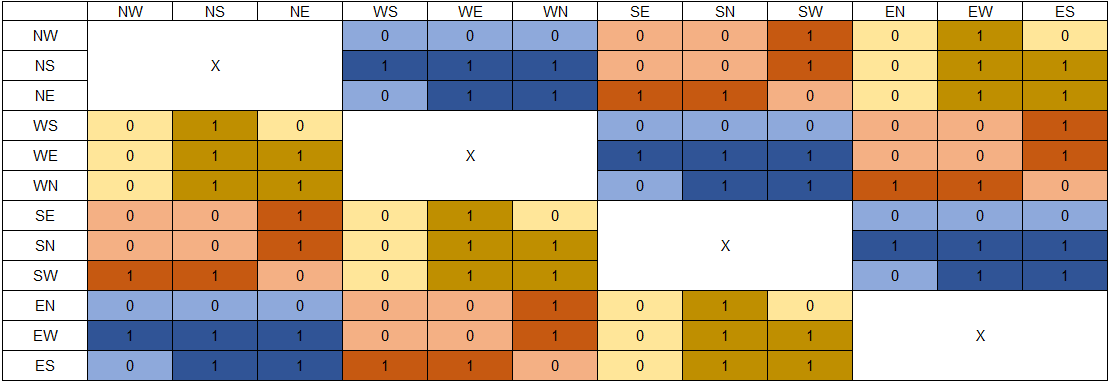
\includegraphics[scale=0.32]{collision table.png}}
    \caption{collision table with relative outputs}
    \label{table}
\end{figure}

Taking this specific concept of collision we noticed that we can simplify the output answers greatly, theoretically we could simplify the answers in three separate output blocks, but in order to have a much more simpler solution to VHDL, we just imagined the whole graph to be mirrored diagonally.


\subsubsection{Code Implementation}

When considering the required IO for our system, since the directions of each car will be represented by 4 bit system - we implemented 8 inputs in total, 4 bit directional representations for the two cars, which collision has to be checked. In terms of an output, we considered the most optimal solution is to have a single output, which would represent weather the collision is present or not.

Later on, we define all of the cardinal directions as signals, dedicating the 4 bit combination of each car to the direction representation. Hence, the original 4 bit input is just to represent the 12 possible directions, from which a car could come from and go to. Since we define that for 2 separate cars, each of them have a unique representation and so overall we have 24 directional signals defined.

Finally, we represent the logic of the collision table to the VHDL by expressing solutions, when the main output is considered to be equals to one. For instance, taking a look at the Figure \ref{table} we see, that if the first car comes from west to south and the second car is coming from north to south, then our collision, in this term our output is one. This is done with a all of the cases, where the collision is considered to happen and as referred before, since the graph is repetitive, only half of the solutions have to be implemented. Hence having this defined concludes the code implementation of VHDL

\subsection{FreeRTOS Implementation}

\subsubsection{The choice of FreeRTOS}

When it comes to software implementation of this project, the most feasible decision was to use the open source FreeRTOS kernel and all its respective libraries. The kernel is mainly C based and it provides many useful and interesting functionalities linked to the implementation and development of real time systems under the software aspect. In our implementation we made use of the FreeRTOS to create our own scheduler which handles two separate Queues of entities. The entities which belong to our system are the cars which enters the system at any not given point in time. The idea is to register the cars as soon as they cross the first line present in the cross section, done so, the cars will be pushed into what we called "Unscheduled Queue". Since the cross section has only 4 lanes with a single line per direction, hence the highest possible number of cars which have to be registered at the same time is 4. The last mentioned case is also assumed to be a worst case scenario since in real life it could be rare to have such situation happening. To solve this problem we created a buffer which is making sure that within a certain time span, 50 ms was set for our scenario, the cars entering the system will be buffered accordingly and sorted into the unscheduled queue. After the scheduler performs some conditions checks in the queues it can finally decide to push the cars into the scheduled queue. At this point it will be needed to check whether the cars are free to go or a collision will happen with a different car in the same system. The detailed explanation of how the scheduling and queues work is handled in the next paragraphs.

\subsubsection{Scheduling and queues}

As already mentioned, two different queues are used in our software. In sequential order, the cars will be first handled and pushed into a buffer which will make sure we can register cars even with a small notice time. This means that if multiple cars cross the line at almost the same time point they will still be sorted inside the queue according to the registration time. For the case to be handled, we came up with the conclusion of using a simple FIFO algorithm, first in, first out, to get rid of the cars according to their arrival time. Now let us take into account a simple scenario in which two cars reach the initial line at t\textsubscript{1} = 12.4 s and t\textsubscript{2} = 12.7 s. In real life the difference will be almost unnoticeable but in a real time system the difference will be highly relevant, therefore setting a delay for the polling time equals to t\textsubscript{p} = 50 ms, makes sure that we can register cars that enter the system as long as the time difference is not smaller than 50 ms. The buffer can only contain maximum 4 cars (worst case scenario), which leads to a maximum buffer filling time of

t\textsubscript{p}\textsuperscript{MAX} = 200 ms, and once it gets full, or the cars will pass through the second line, the information received will be pushed to the unscheduled queue and the buffer will be emptied and reset. From this point, 3 possible cases can happen:

\begin{figure*}[ht]
\centering{\includegraphics[scale=0.45]{TestBench_Results.png}}
    \caption{Waveform of all of the possible outcomes of Traffic Controller}
    \label{testbench}
\end{figure*}

\begin{enumerate}
\item The cars will be assumed to need a certain amount of time before reaching the second line, hence, once they reach the line, the buffer will be emptied automatically and the cars moved to the scheduled queue.

\item The buffer has been filled even before the first car registered crossed the second line, therefore the cars will be automatically pushed into the scheduled queue after a short time delay and the unscheduled queue will be emptied.

\item A 5th car enters the system before the unscheduled queue is emptied, therefore the cars will be preemptively pushed into the scheduled queue and the unscheduled queue will be emptied to make space for the new cars registering, with a short time delay.
\end{enumerate}

By handling these 2 possible cases, we make sure that there will always be space for registering new cars approaching and, if no major accidents happen, the scheduler will keep doing its job periodically.
A snippet of code will be shown below in order to understand how the algorithm formally works.
[insert picture of scheduling algorithm]

\subsubsection{Communication}



\section{Simulation Results}

\subsection{ModelSIM results}

Considering the results of our already written VHDL representation of the collision checking, which we in the end decided to call - Traffic Controller, we noticed, that simulating the code itself, the answers were corresponding to the collision table and testing the inputs one by one, we saw that the code was working as it intended, but to represent all of the inputs correspondingly and truly showing, that the solution works, was not as easy we initially thought.

To really prove, that all of the collisions were realised in our system, we had to create a test-bench, which worked as follows: since single cars direction is represented with 4 unique inputs, one set of inputs were considered as a fixed value, while other set of inputs was running through all of the possible outcomes. After doing that we increase the value of the fixed set by one and run all of the possible outcomes with the other set again. This has been done throughout all of the values, which we use as directions, which means, that the combinations "1100", "1101", "1110", "1111" were not considered, but since the system is designed to output a 0 at all of the other undefined outputs, the outcome would just be 0 at the output through these values. Essentially we simulated all of the possible outcomes, shown in the Table \ref{table}, even considering the areas marked as "X".

The exact simulation results of this described test-bench are shown in the Figure \ref{testbench}. Inputs from 'a' to 'd' in alphabetical order represent the change of the fixed sets values, when the inputs from 'e' to 'h' also in alphabetical order represent changing set of values. Variable 'x' is the output, which represents collision status, if it is equal to one - the collision is detected.

\begin{thebibliography}{00}
\bibitem{b1} G. Eason, B. Noble, and I. N. Sneddon, ``On certain integrals of Lipschitz-Hankel type involving products of Bessel functions,'' Phil. Trans. Roy. Soc. London, vol. A247, pp. 529--551, April 1955.
\bibitem{b2} J. Clerk Maxwell, A Treatise on Electricity and Magnetism, 3rd ed., vol. 2. Oxford: Clarendon, 1892, pp.68--73.
\bibitem{b3} I. S. Jacobs and C. P. Bean, ``Fine particles, thin films and exchange anisotropy,'' in Magnetism, vol. III, G. T. Rado and H. Suhl, Eds. New York: Academic, 1963, pp. 271--350.
\bibitem{b4} K. Elissa, ``Title of paper if known,'' unpublished.
\bibitem{b5} R. Nicole, ``Title of paper with only first word capitalized,'' J. Name Stand. Abbrev., in press.
\bibitem{b6} Y. Yorozu, M. Hirano, K. Oka, and Y. Tagawa, ``Electron spectroscopy studies on magneto-optical media and plastic substrate interface,'' IEEE Transl. J. Magn. Japan, vol. 2, pp. 740--741, August 1987 [Digests 9th Annual Conf. Magnetics Japan, p. 301, 1982].
\bibitem{b7} M. Young, The Technical Writer's Handbook. Mill Valley, CA: University Science, 1989.
\end{thebibliography}

\end{document}